\section{Техническое задание}


\subsection{Основание для разработки}
Основанием для разработки является задание на выпускную квалификационную работу бакалавра "<Программно-информационная система оптимизации ресторанного бизнеса">.

\subsection{Цель и назначение разработки}
Основной задачей выпускной квалификационной работы является разработка программы для оптимизации ресторанного бизнеса. Для достижения поставленной цели необходимо решить следующие задачи: 
\begin{itemize}
	\item провести анализ предметной области; 
	\item разработать концептуальную модель программы; 
	\item спроектировать базу данных;
	\item разработать механизм формирования финансовых отчётов;
	\item реализовать процесс создания технологических карт;
	\item интегрировать данные сотрудников в систему.
\end{itemize}

\subsection{Требования пользователя к интерфейсу программы}
Программа должна включать в себя:
\begin{itemize}
    \item авторизацию;
    \item доступы для управляющего, администратора, повара, официант;
    \item окно ввода заказа;
    \item модуль для управления данными сотрудников;
    \item возможность создания технологических карт;
    \item формирование финансовых отчётов.
\end{itemize}

Композиция шаблона окна авторизации представлена на рисунке ~\ref{compositionin:image} и состоит из:
\begin{itemize}
	\item поле для ввода кода (1);
	\item экранная клавиатура (2);
	\item кнопка для очистки поля (3);
	\item кнопка для подтверждения ввода пароля (4).
\end{itemize}
\begin{figure}[ht]
	\centering
	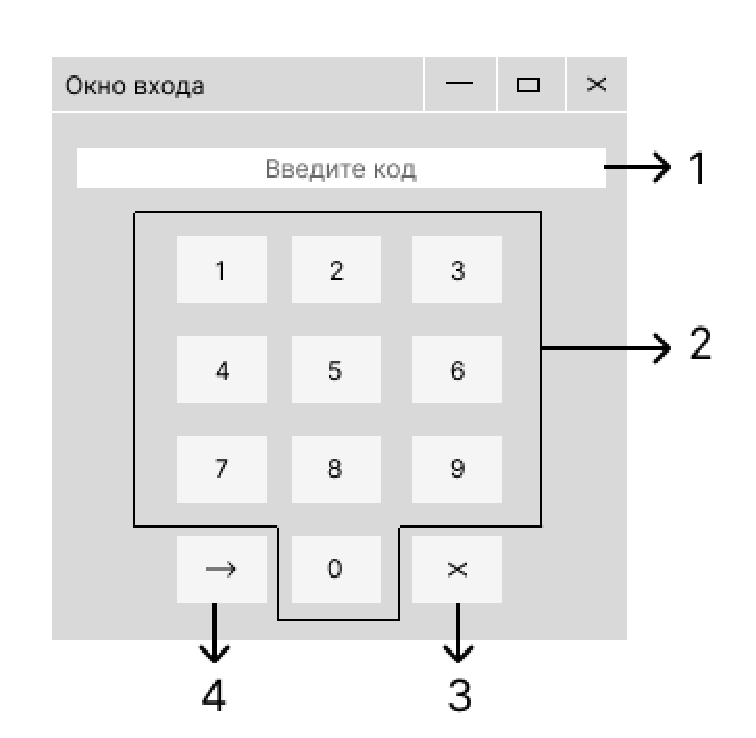
\includegraphics[width=0.5\linewidth]{compositionin}
	\caption{Композиция шаблона окна авторизации}
	\label{compositionin:image}
\end{figure}

Схема окна ввода заказа продемонстрирована на рисунке ~\ref{compositionzakaz:image} и содержит следующие компоненты:
\begin{itemize}
	\item поле для вывода номера заказа и стола (1);
	\item таблицы вывода данных о блюдах (2);
	\item кнопка для добавления скидки (3);
	\item поле для подсчёта итоговой стоимости (4);
	\item кнопка для печати заказа (5);
	\item кнопка для оплаты заказа(6);
	\item кнопки с названием блюда для добавления их в заказ (7);
	\item кнопки с названием категорий для выбора блюд (8).
\end{itemize}
\begin{figure}[ht]
	\centering
	\includegraphics[width=0.8\linewidth]{compositionzakaz}
	\caption{Композиция шаблона окна заказа}
	\label{compositionzakaz:image}
\end{figure} 

\newpage
Шаблон модуля для работы с базой данных (управление данными сотрудников, редактирование меню) изображен на рисунке ~\ref{composition1:image}. Он включает в себя:
\begin{itemize}
	\item кнопка для добавления данных (1);
	\item кнопка для редактирования данных (2);
	\item кнопка для удаления данных (3);
	\item кнопка для поиска данных (4);
	\item кнопка для поиска в таблице (5);
	\item таблица для просмотра данных из БД (6).
\end{itemize}
\begin{figure}[ht]
	\centering
	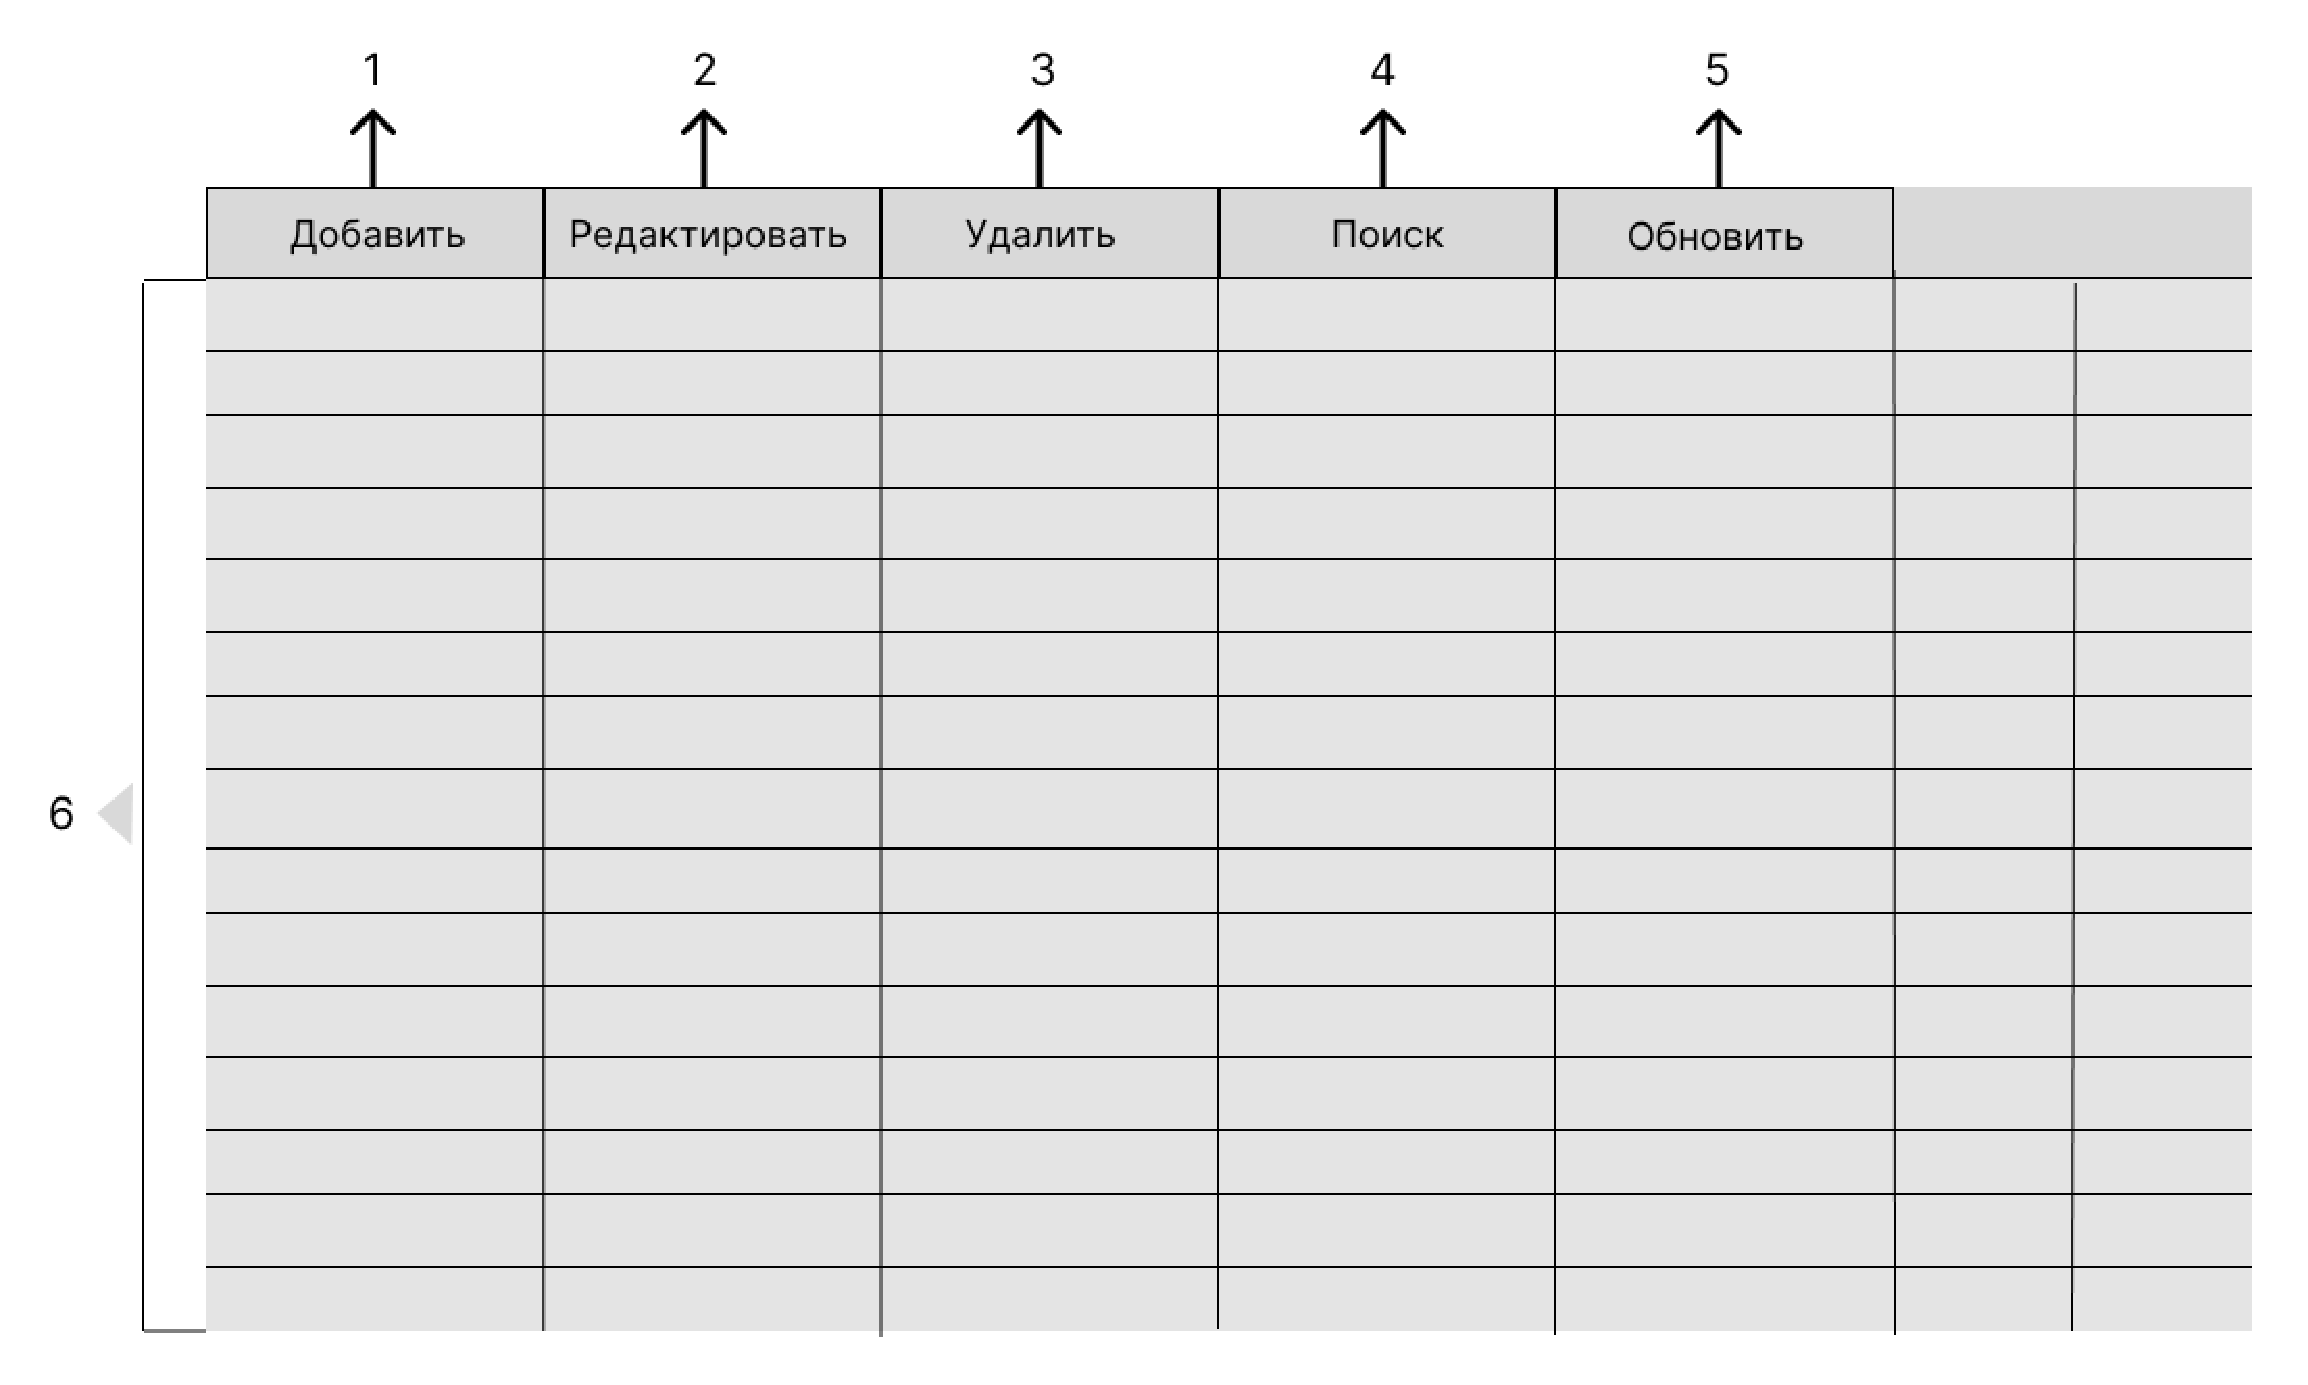
\includegraphics[width=0.7\linewidth]{composition1}
	\caption{Композиция шаблона модуля работы с базой данных}
	\label{composition1:image}
\end{figure}

\newpage
Макет окна для создания технологических карт проиллюстрирован на рисунке ~\ref{compositiontex:image} и состоит из:
\begin{itemize}
	\item поле для ввода названия блюда (1);
	\item поле для ввода описания блюда (2);
	\item поле для ввода рецепта (3);
	\item кнопка для редактирования данных ингредиентов в таблице (4);
	\item кнопка для добавления ингредиентов в таблицу (5);
	\item таблица для добавления данных об ингредиентах (6);
	\item поле для ввода количества белков (7);
	\item поле для ввода количества жиров (8);
	\item поле для ввода количества углеводов (9);
	\item поле для ввода количества калорий (10);
	\item кнопка для сохранения данных в БД (11);
	\item кнопка для удаления данных из таблицы ингредиентов (12);
\end{itemize}
\begin{figure}[ht]
	\centering
	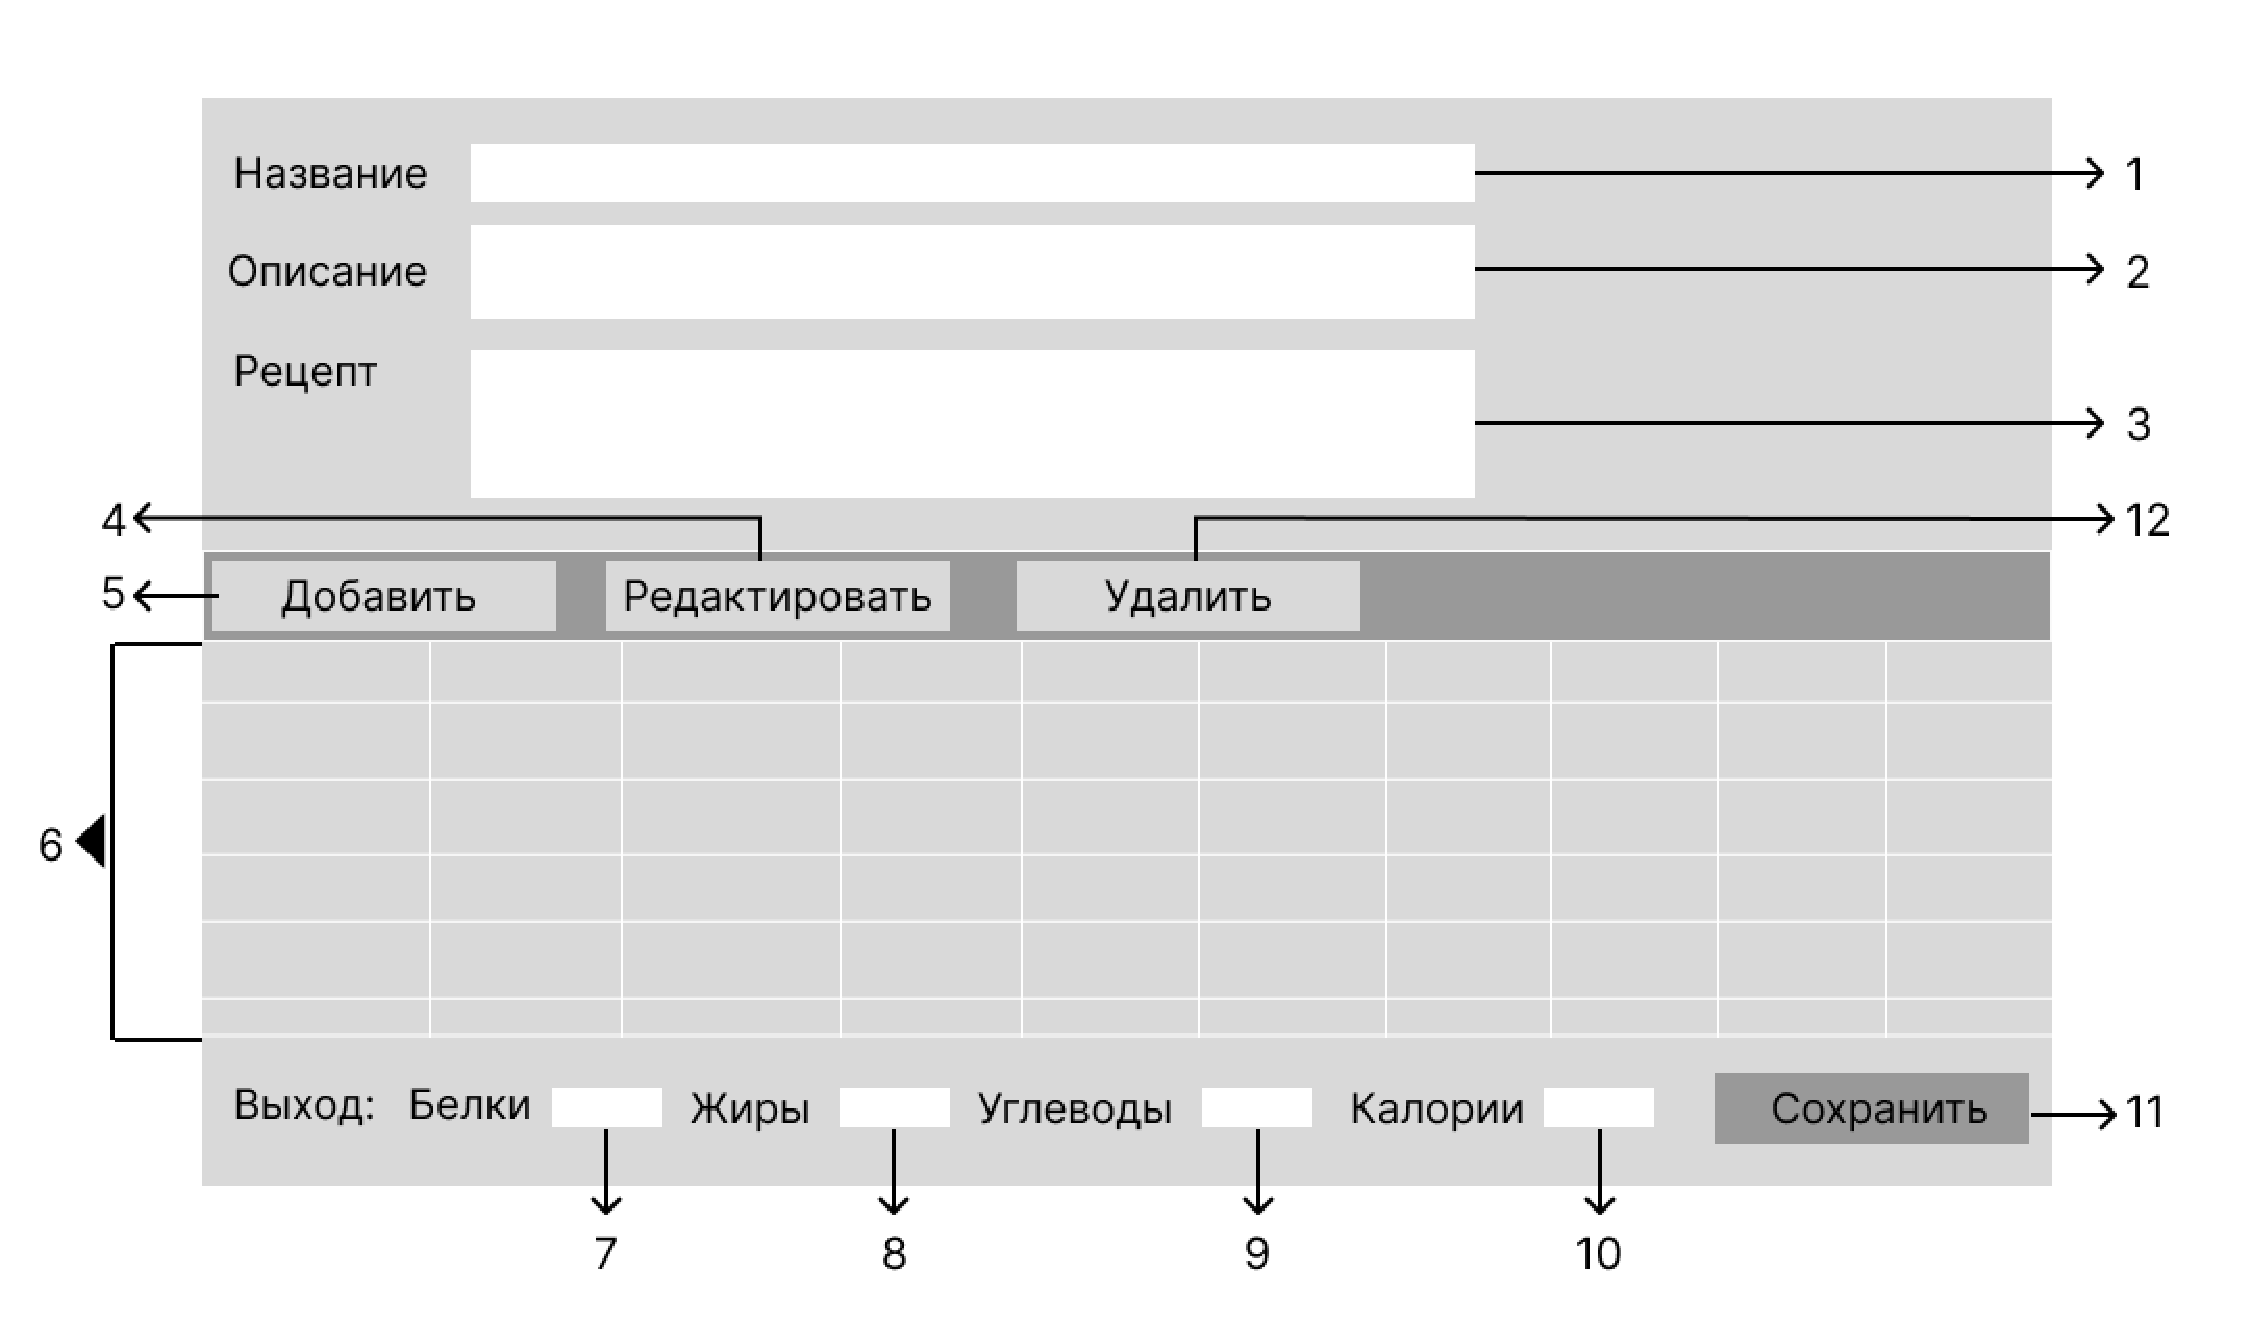
\includegraphics[width=0.8\linewidth]{compositiontex}
	\caption{Композиция шаблона модуля для создания технологических карт}
	\label{compositiontex:image}
\end{figure}


\newpage
\subsection{Моделирование вариантов использования}

Для разрабатываемой системы была реализована модель, обеспечивающая наглядное представление вариантов использования программы с помощью унифицированного языка визуального моделирования UML. 

В диаграмме вариантов (прецедентов) проектируемая система рассматривается как ряд прецедентов, предоставляемых системой актерами - пользователями или другими компьютерными системами, взаимодействующими с данной. Варианты использования системы изображаются в виде овалов, внутри которых пишется название сценария \cite{uml}. Сценарий взаимодействия позволяет пользователям достигать целей использования программы с помощью функциональной системы. Связь между актёрами и вариантами использования реализуют с помощью ассоциаций. 

Использование UML для визуального представления работы системы позволяет выявить ключевые взаимодействия и зависимости между элементами программы, что упрощает понимание требований и возможностей системы, а также способствует более эффективной разработке и тестированию. 

На основании анализа предметной области в программе должны быть реализованы следующие прецеденты:
\begin{enumerate}
\item Добавление, просмотр и редактирование данных о сотруднике.
\item Создание, просмотр и редактирование заказа.
\item Создание, просмотр и редактирование технологических карт.
\item Обработка платежа.
\item Создание и просмотр финансовых отчётов.
\end{enumerate}

Программа имеет четыре группы пользователей с разными правами: управляющий, старший повар, администратор и официант. 
\newline
Управляющему должны быть доступны следующие функции:
\begin{enumerate}
	\item Добавление, просмотр и редактирование данных о сотрудниках.
	\item Создание, просмотр и редактирование данных о должностях.
	\item Редактирование данных заведения.
	\item Управление количеством столов.
	\item Редактирование типов оплаты.
	\item Назначение размеров скидки.
\end{enumerate}
На рисунке ~\ref{diagramyprav:image} изображены прецеденты для управляющего.
\begin{figure}[ht]
	\centering
	\includegraphics[width=1\linewidth]{diagramyprav}
	\caption{Диаграмма прецедентов для категории пользователей - управляющий}
	\label{diagramyprav:image}
\end{figure}
\newline
Старшему повару должны быть доступны следующие функции:
\begin{enumerate}
	\item Добавление, просмотр и редактирование данных о блюдах.
	\item Создание, просмотр и редактирование технологических карт.
	\item Добавление категорий меню.
	\item Добавление ингредиентов.
\end{enumerate}
На рисунке ~\ref{diagramlshef:image} изображены прецеденты для старшего повара.
\begin{figure}[ht]
	\centering
	\includegraphics[width=1\linewidth]{diagramlshef}
	\caption{Диаграмма прецедентов для категории пользователей - старший повар}
	\label{diagramlshef:image}
\end{figure}
\newpage
Официанту должны быть доступны следующие функции:
\begin{enumerate}
	\item Создание, редактирование, удаление заказа.
	\item Передача заказа на кухню.
	\item Формирование счёта.
	\item Обработка оплаты.
	
\end{enumerate}
На рисунке ~\ref{diagramoff:image} изображены прецеденты для официанта ресторана.
\begin{figure}[ht]
	\centering
	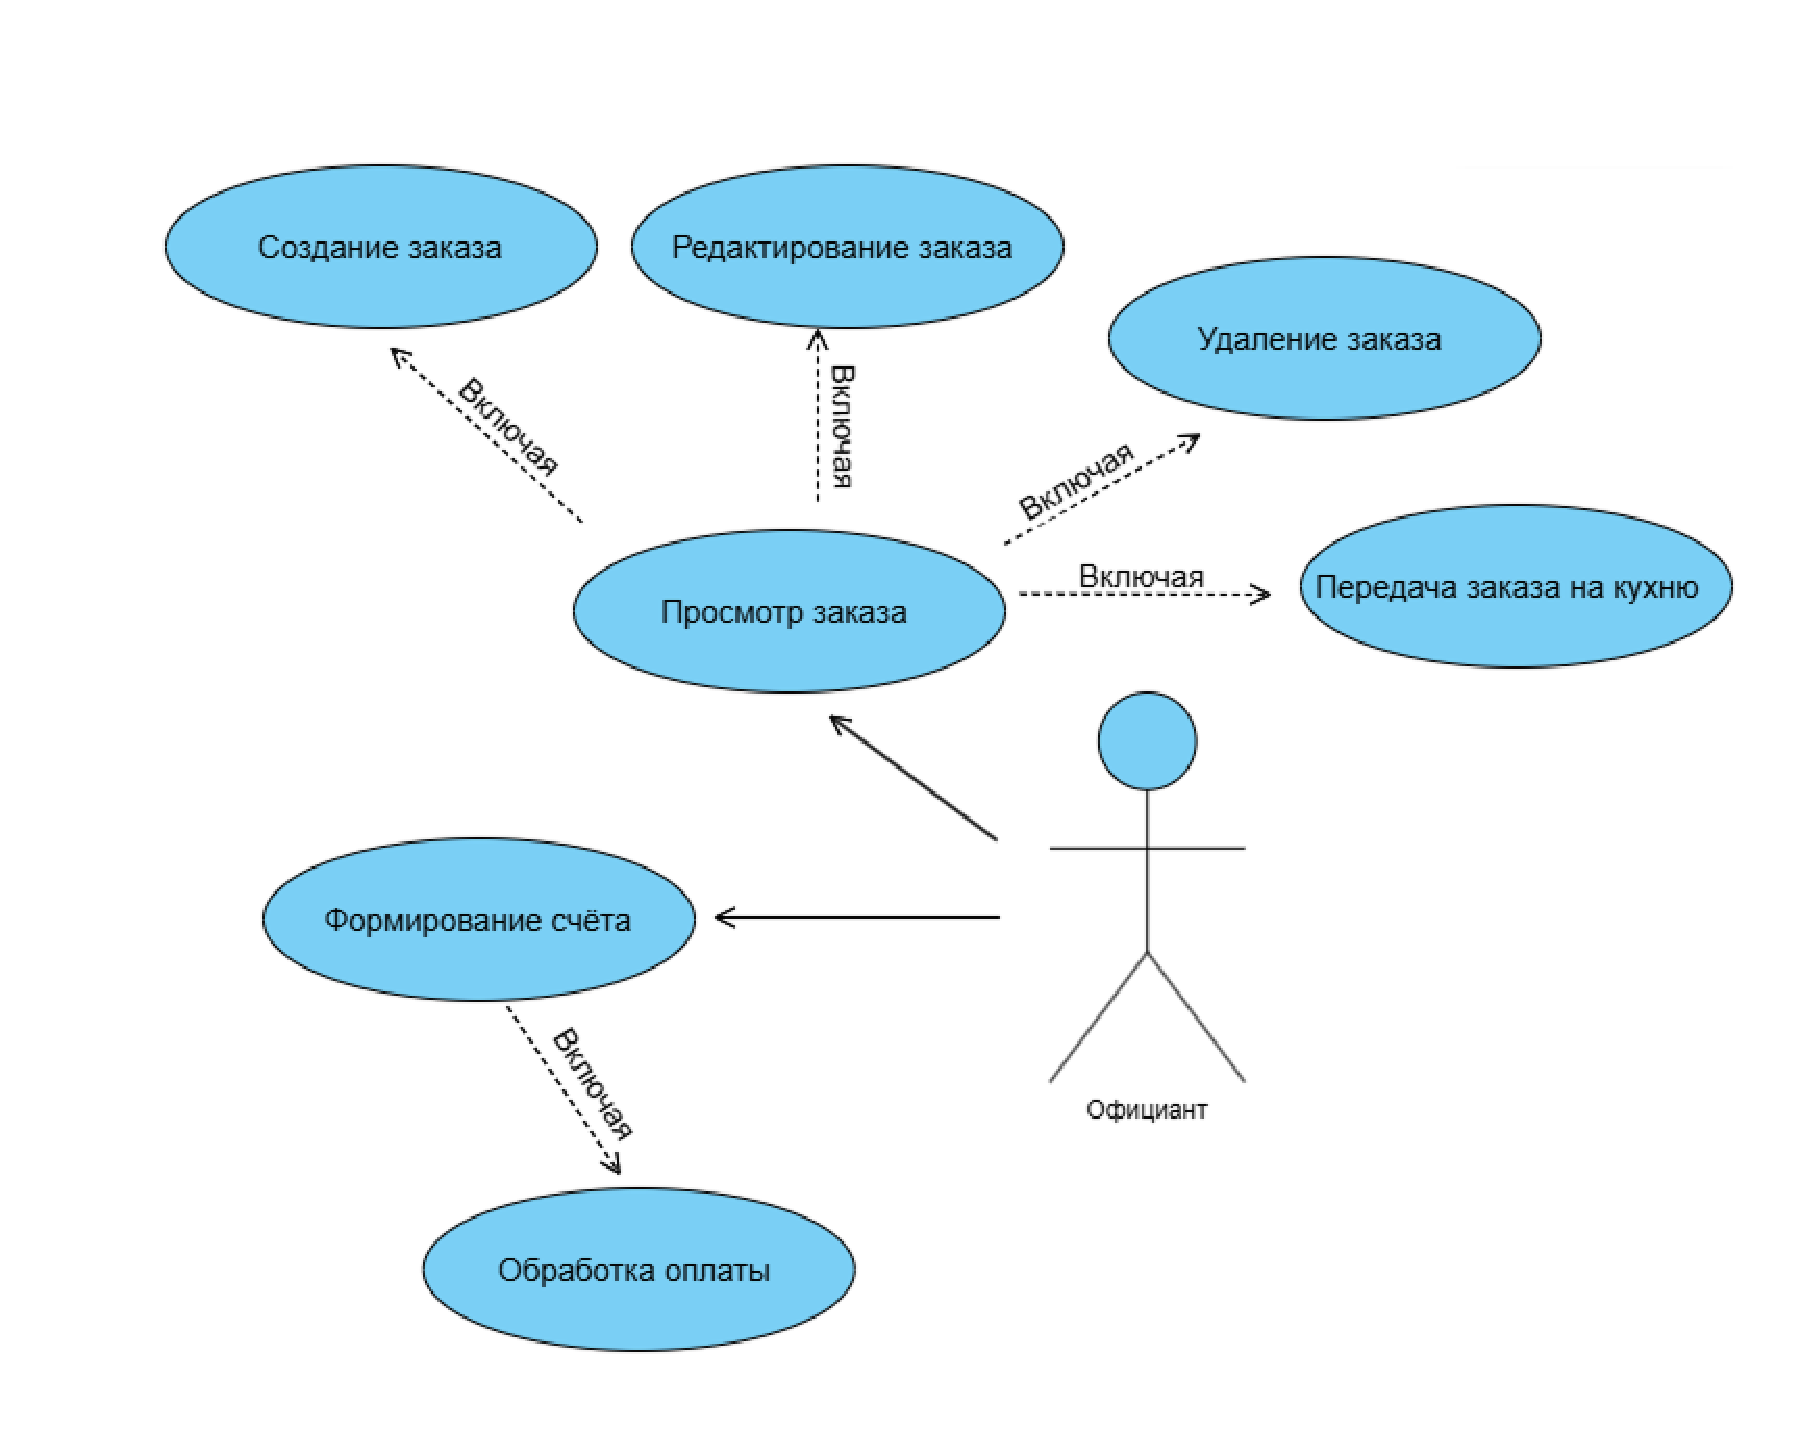
\includegraphics[width=1\linewidth]{diagramoff}
	\caption{Диаграмма прецедентов для категории пользователей - официант}
	\label{diagramoff:image}
\end{figure}
\newpage
Администратору должны быть доступны следующие функции:
\begin{enumerate}
	\item Просмотр отчёта о закрытии смены.
	\item Просмотр отчёта о движении денежных средств.
	\item Просмотр данных закрытых заказов.
\end{enumerate}
На рисунке ~\ref{diagramadmin:image} изображены прецеденты для администратора ресторана.
\begin{figure}[ht]
	\centering
	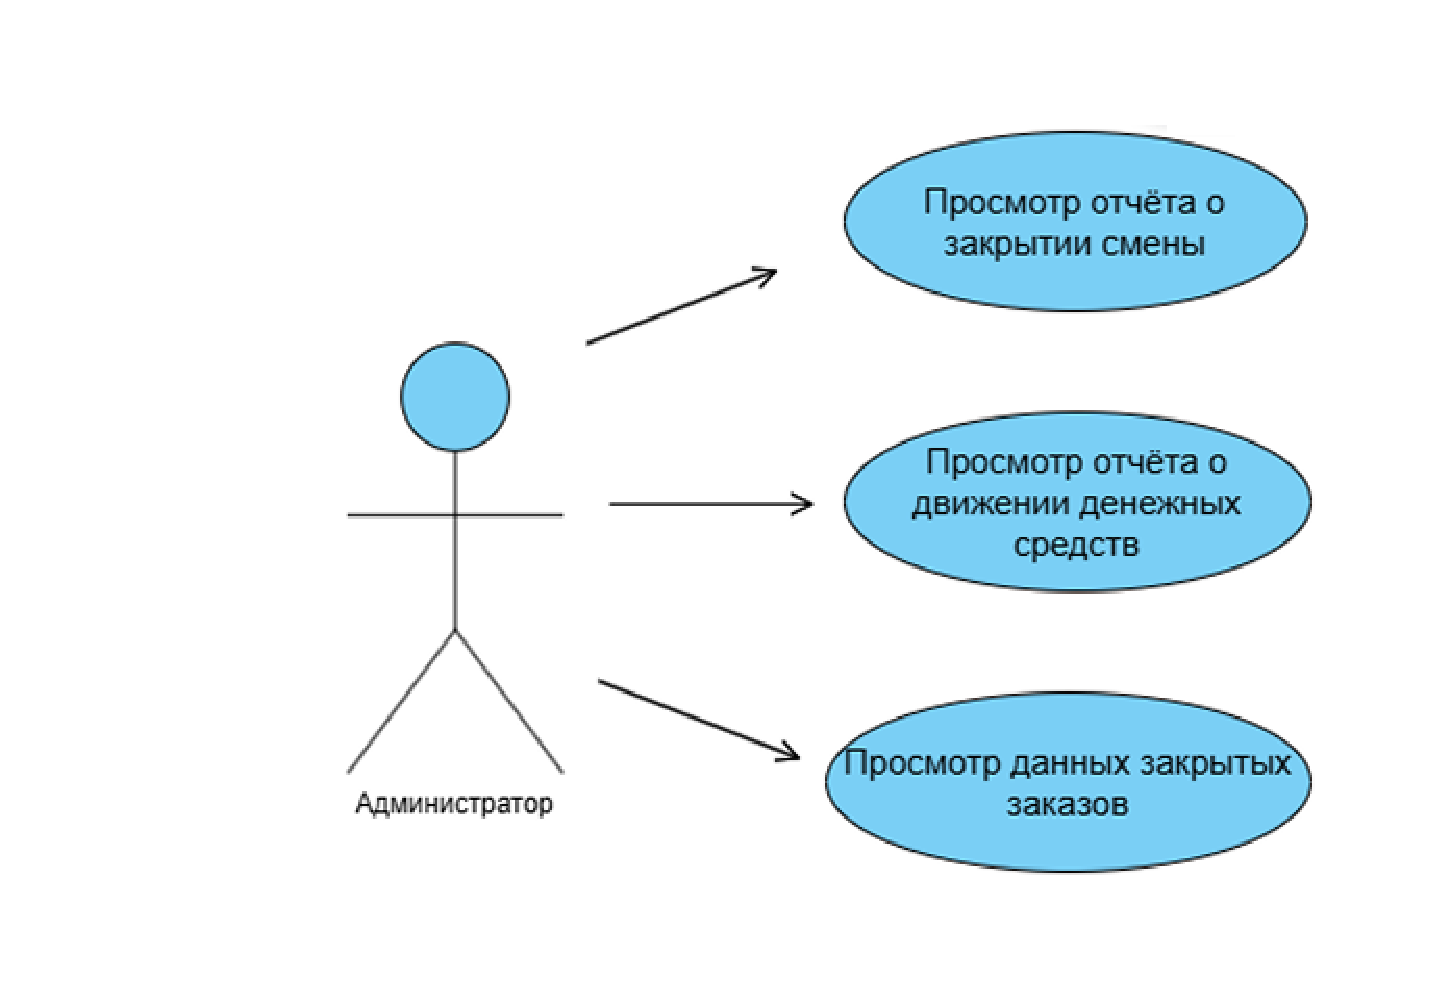
\includegraphics[width=0.7\linewidth]{diagramadmin}
	\caption{Диаграмма прецедентов для категории пользователей - администратор}
	\label{diagramadmin:image}
\end{figure}


\newpage
\subsection{Требования к оформлению документации}

Разработка программной документации и программного изделия должна производиться согласно ГОСТ 19.102-77 и ГОСТ 34.601-90. Единая система программной документации.
